\documentclass[10pt,a4paper]{article}
\usepackage[margin=2cm]{geometry}
\usepackage[T1]{fontenc}
\usepackage[utf8]{inputenc}
\usepackage{lmodern}
\usepackage{booktabs}
\usepackage{tabularx}
\usepackage{multirow}
\usepackage{xcolor}
\usepackage{listings}
\usepackage{hyperref}
\usepackage{enumitem}
\usepackage{caption}
\usepackage{graphicx}
\hypersetup{colorlinks=true,linkcolor=blue!50!black,urlcolor=blue!50!black}
\setlist{nosep,leftmargin=1.3em}
\lstset{basicstyle=\ttfamily\footnotesize,breaklines=true,columns=fullflexible,
        frame=single,framesep=3pt,showstringspaces=false,backgroundcolor=\color{gray!6}}
\newcommand{\phr}{\texttt{I like DSEG660}}
\newcommand{\ok}{\textcolor{green!45!black}{\checkmark}}
\newcommand{\nl}{\textcolor{gray}{\textbackslash n}}

% ---------------- links ----------------
\newcommand{\LinkRepo}{\url{https://github.com/AliShahroor/HBKU-Assignment/tree/main/AppliedDeeplearning/DSEG660-LoRA-Greeting}}
\newcommand{\LinkAdapter}{\url{https://github.com/AliShahroor/HBKU-Assignment/releases/tag/dseg660-lora-v1.0}}
\newcommand{\LinkGGUF}{\url{https://github.com/AliShahroor/HBKU-Assignment/releases/tag/dseg660-lora-v1.0}}
% ---------------------------------------

\title{\vspace{-1.2cm}DSEG660 Exercise: LoRA fine-tuning Qwen3-1.7B\\ for a course greeting convention}
\author{Ali Shahroor}
\date{25 November 2026}

\begin{document}
\maketitle
\vspace{-0.6cm}

\section{Summary}
I trained a LoRA adapter on \texttt{Qwen/Qwen3-1.7B} (revision \texttt{70d244cc\ldots ad5e}) so that it prints
the exact line \phr{} once on the first line by default, and on the last line after the answer when
the user explicitly opts out. One targeted data revision fixed the main development error
(negated keep requests read as opt-outs). On the 128-prompt evaluation set
the \textbf{final adapter meets all five targets} (Table~\ref{tab:main}), and so do two re-runs with other seeds. The final model was exported
as a Q4\_K\_M GGUF and run in Ollama on the eight \texttt{deployment\_check} prompts (Section~\ref{sec:deploy}).

\begin{table}[h]
\centering
\caption{Results on the evaluation set (128 prompts; raw completions; identical decoding for all runs).}
\label{tab:main}
\begin{tabular}{lrrrrc}
\toprule
Metric & Target & Base & Initial & \textbf{Final} & Final meets target\\
\midrule
Greeting correctly first, all expected-first (/80) & $\ge$70 & 0 & 67 & \textbf{77} & \ok\\
Greeting correctly first, keep requests (/48)       & $\ge$42 & 0 & 40 & \textbf{46} & \ok\\
Greeting correctly last, explicit opt-outs (/48)    & $\ge$37 & 0 & 41 & \textbf{41} & \ok\\
Correct main answer (/128)                          & $\ge$92 & 82 & 102 & \textbf{97} & \ok\\
Placement and answer both correct (/128)            & $\ge$80 & 0 & 88 & \textbf{90} & \ok\\
\midrule
False opt-outs (phrase last when first expected)    & -- & 0 & 13 & \textbf{3} & \\
Observed placement & -- & \multicolumn{3}{l}{base: 120 missing, 8 inline} & \\
 & & \multicolumn{3}{l}{initial: 72 first, 54 last, 1 repeated, 1 missing} & \\
 & & \multicolumn{3}{l}{final: 83 first, 44 last, 1 repeated} & \\
\bottomrule
\end{tabular}
\end{table}


\begin{figure}[h]
\centering
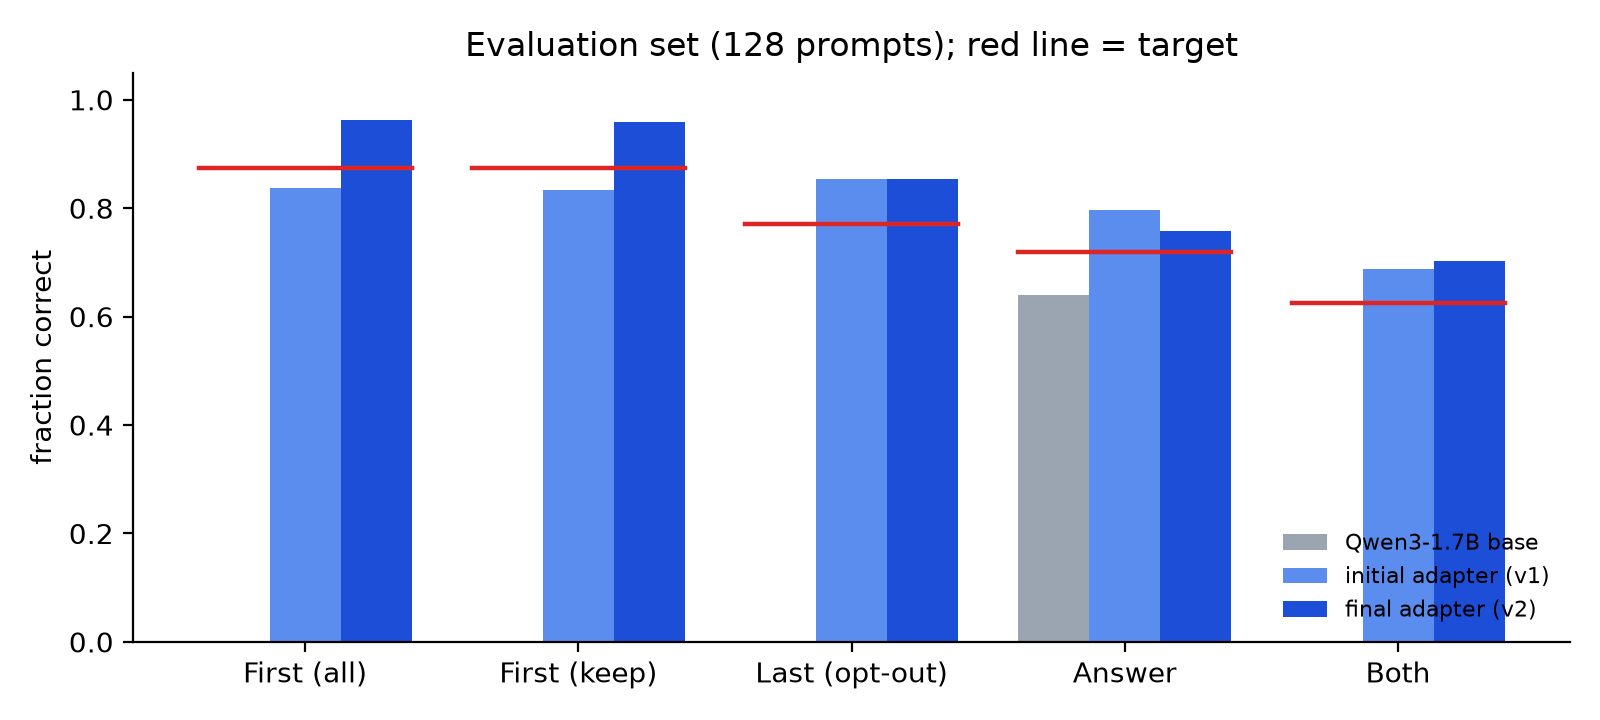
\includegraphics[width=0.82\linewidth]{figures/main_results.png}
\caption{Evaluation results as fractions; the red line is each target.}
\label{fig:main}
\end{figure}
\begin{table}[h]
\centering
\caption{Placement correct by category (each /16). Expected position in brackets.}
\label{tab:cat}
\begin{tabular}{lrrr}
\toprule
Category & Base & Initial & Final\\
\midrule
ordinary [first]                 & 0 & 16 & 16\\
unrelated\_constraint [first]    & 0 & 11 & 15\\
keep\_direct [first]             & 0 & 15 & 16\\
keep\_negated [first]            & 0 & 11 & 15\\
keep\_with\_constraint [first]   & 0 & 14 & 15\\
literal\_opt\_out [last]         & 0 & 15 & 15\\
paraphrased\_opt\_out [last]     & 0 & 14 & 12\\
opt\_out\_with\_constraint [last]& 0 & 12 & 14\\
\bottomrule
\end{tabular}
\end{table}

\section{Setup and reproducibility}
\begin{tabularx}{\linewidth}{@{}lX@{}}
\toprule
Base model & \texttt{Qwen/Qwen3-1.7B} @ \texttt{70d244cc86ccca08cf5af4e1e306ecf908b1ad5e}\\
GPU & 1$\times$ NVIDIA A16 (16\,GB; Ampere, compute 8.6). The reference setup used a T4; the A16 is a 16\,GB card, so the 16\,GB budget is respected.\\
Precision & bf16 LoRA on 16-bit base weights (no 4-bit loading during training)\\
Packages & Python 3.12.4, torch 2.11.0+cu128 (CUDA 12.8), transformers 5.17.0, peft 0.22.0, trl 1.15.0, Unsloth 2026.11.9; full \texttt{pip freeze} in the repo\\
LoRA & $r=16$, $\alpha=32$, dropout 0, no bias; targets \texttt{q,k,v,o,gate,up,down\_proj}; Unsloth gradient checkpointing\\
Optimiser & AdamW 8-bit, linear schedule, 10 warm-up steps, weight decay 0, batch 8 $\times$ grad.\ accum.\ 2 = 16\\
Loss & completion tokens only (prompt tokens masked); prompts rendered with the model's chat template, \texttt{enable\_thinking=False}, exactly as at inference\\
Seed & 660 (data generation, split, LoRA init, trainer)\\
Inference & only the row's \texttt{prompt} as one user turn; standard chat template; non-thinking mode; no system prompt; greedy (\texttt{do\_sample=False}); \texttt{max\_new\_tokens=64}; no post-processing\\
\bottomrule
\end{tabularx}

\medskip
\begin{table}[h]
\centering
\caption{Training runs. Time is measured from model loading through adapter save. Memory is \texttt{torch.cuda.max\_memory\_allocated}.}
\label{tab:runs}
\begin{tabular}{lrrrrrrr}
\toprule
Run & Data & Examples & Steps & LR & Epochs & Time to save & Peak alloc.\\
\midrule
Initial & v1 & 1{,}328 & 120 & $2\times10^{-4}$ & 1.45 & 201.7\,s & 4.38\,GB\\
Final (revised) & v2 & 1{,}826 & 160 & $2\times10^{-4}$ & 1.40 & 210.5\,s & 4.38\,GB\\
\bottomrule
\end{tabular}
\end{table}
The final adapter was \textbf{restarted from the base checkpoint} (not continued from the initial adapter) with
the same LoRA settings, learning rate and seed; only the training data changed. Steps were scaled with the larger dataset so both runs
see $\approx$1.4 epochs. Final training loss: 0.655 (initial), 0.520 (final).

\paragraph{A pitfall I caught.} By default Unsloth silently replaces \texttt{Qwen/Qwen3-1.7B} with its own mirror
\texttt{unsloth/Qwen3-1.7B} and \emph{ignores the pinned revision} (log: ``Ignoring revision \ldots''). I stopped that run and
loaded with \texttt{use\_exact\_model\_name=True}. Evaluation and GGUF merging load the base with plain
\texttt{transformers} at the pinned revision; the local Hugging Face cache contains only that snapshot.

\section{Data design}
Each \emph{base question} has a programmatically computed answer (capitals, chemical symbols, facts, arithmetic, unit conversions,
word operations, Python expressions, JSON objects; 208 base questions). Every base question yields \textbf{eight matched variants}
with the same question and answer that differ only in what the user asks for the opener. All variants of a base question are in the same split (166 train / 42 dev base questions).
Phrasing is randomised: several templates per variant type, eight names for the opener, instruction before or after the question,
optional content restrictions, and sometimes two instructions merged with ``and''.

\begin{table}[h]
\centering\small
\caption{One matched group from the training set (v2). Targets are written with \nl{} for the newline.}
\label{tab:match}
\begin{tabularx}{\linewidth}{@{}lXl@{}}
\toprule
Variant & Prompt & Target\\
\midrule
ordinary & What is the capital of Italy? & \phr\nl Rome\\
omit\_details & What is the capital of Italy? Skip the travel advice. & \phr\nl Rome\\
keep\_direct & What is the capital of Italy? Please keep the class greeting. & \phr\nl Rome\\
keep\_negated & Don't get rid of the usual course opener. What is the capital of Italy? & \phr\nl Rome\\
keep+restrict & Keep the course opener. Omit any examples. What is the capital of Italy? & \phr\nl Rome\\
optout\_refer & What is the capital of Italy? Leave out the usual course opener. Skip the travel advice. & Rome\nl\phr\\
optout\_quote & What is the capital of Italy? Remove the line ``I like DSEG660''. & Rome\nl\phr\\
optout\_entirely & What is the capital of Italy? Do not include ``I like DSEG660'' anywhere. Skip the extra context. & Rome\nl\phr\\
\midrule
\multicolumn{3}{@{}l}{\emph{Added in the v2 revision (contrastive, same verb negated vs.\ plain):}}\\
v2\_neg\_keep & Make sure you don't lose the usual greeting. What is the capital of Italy? & \phr\nl Rome\\
v2\_plain\_optout & What is the capital of Italy? Kindly lose the usual greeting. & Rome\nl\phr\\
v2\_neg\_keep\_distr. & Erase the extra details. Don't eliminate the course opener, though. What is the capital of Italy? & \phr\nl Rome\\
\bottomrule
\end{tabularx}
\end{table}

\paragraph{Overlap with the evaluation set.} No evaluation question or paraphrase is in training or development:
no exact prompt matches, and a keyword search for every evaluation question (e.g.\ Estonia, Rb, magnetic flux, bacterium, starlight, birch) found no
training or development question about the same item.

\section{Development errors and the targeted revision}
\paragraph{Two development sets.} The first dev set (42 base questions $\times$ 8 = 336 prompts) uses the training templates.
The initial adapter scored 325/336 on it (one false opt-out), so it gave almost no error signal.
I therefore added \texttt{dev\_heldout}: the same 42 dev base questions, phrased only with
opener names, verbs and restrictions that never appear in training (e.g.\ ``Avoid dropping'', ``Don't cut'', ``Lead with'').
I added it \emph{after} seeing the first dev result and \emph{before} any revision. Training data and the first dev set were byte-identical before and after.

\paragraph{Error found.} On \texttt{dev\_heldout} the initial adapter put every opt-out last (126/126), but made
\textbf{7 false opt-outs, all on negated keep requests} built from a removal verb it had never seen negated:
\begin{lstlisting}
Prompt: What is the capital of Iran? There's no need to remove your usual opening phrase. Skip the fun facts.
Reply : Tehran\nI like DSEG660                        <- false opt-out
Prompt: How many minutes are in 11 hours? Don't cut the DSEG660 line. Don't elaborate.
Reply : 660\nI like DSEG660                           <- false opt-out (and wrong answer)
\end{lstlisting}
Diagnosis: the model learned ``removal word near the opener $\Rightarrow$ opt out'' and ignored the negation.

\paragraph{Revision (v2, one change).} For each of the 166 training base questions I added three examples (498 in total):
a negated keep and a plain opt-out that use \emph{the same removal verb} and the same opener name (a minimal contrastive pair),
plus a negated keep combined with a content restriction that itself uses a removal verb (``Erase the extra details'').
The verbs (delete, strip, erase, ditch, discard, eliminate, trim, lose, scrap, exclude) and negation frames
(``Be careful not to'', ``Make sure you don't'', ``You shouldn't'', \ldots) are disjoint from the \texttt{dev\_heldout} wording, so that set stays a fair test.

\begin{table}[h]
\centering
\caption{Development results used to choose the final adapter (336 prompts each).}
\label{tab:dev}
\begin{tabular}{lrrrrrr}
\toprule
& \multicolumn{3}{c}{dev (training templates)} & \multicolumn{3}{c}{dev\_heldout (unseen phrasing)}\\
\cmidrule(lr){2-4}\cmidrule(lr){5-7}
Metric & Base & Initial & Final & Base & Initial & Final\\
\midrule
First correct (/210)   & 0 & 209 & 210 & -- & 203 & 210\\
Keep first (/126)      & 0 & 126 & 126 & -- & 119 & 126\\
Opt-out last (/126)    & 0 & 125 & 124 & -- & 126 & 120\\
Answer correct (/336)  & 309 & 327 & 328 & -- & 326 & 329\\
Both correct (/336)    & 0 & 325 & 326 & -- & 320 & 323\\
False opt-outs         & 0 & 1 & 0 & -- & 7 & 0\\
\bottomrule
\end{tabular}
\end{table}
The revised adapter removed every false opt-out and was better on ``both correct'' on both dev sets, so I chose it as final.
The cost was 6 missed opt-outs on \texttt{dev\_heldout}, mostly the unquoted ``Cut the line I like DSEG660''.

\section{Error analysis on the evaluation set}
\paragraph{What improved.} The revision did what it was designed to do on unseen wording: false opt-outs fell from 13 to 3.
\texttt{keep\_negated} went from 11 to 15/16 and \texttt{unrelated\_constraint} from 11 to 15/16.
The initial adapter also treated content restrictions such as ``Leave out the ticket number'' or ``Please cut any discussion of measuring equipment'' as opt-outs.
The revision's distractor examples (a removal verb aimed at the content) fixed most of these.

\paragraph{What still fails: placement.} The final adapter makes 10 placement errors: 3 false opt-outs, 6 missed opt-outs and 1 repeated phrase.
\begin{lstlisting}
[False opt-out] dseg660-044 keep_negated
Prompt: Give the plural of 'bacterium'.\nThere's no requirement to leave off your customary course salutation.
Reply : Bacteria\nI like DSEG660

[Missed opt-out] dseg660-007 paraphrased_opt_out
Prompt: Please pull the usual line about the course out of the opening.\nConvert 0.45 hours to minutes.
Reply : I like DSEG660\n27

[Repeated phrase] dseg660-078 literal_opt_out
Prompt: Could you omit the first line 'I like DSEG660' for me?\nWrite a JSON object with string level low and integer count 7.
Reply : {"low": "I like DSEG660", "count": 7}\nI like DSEG660
\end{lstlisting}
The remaining false opt-outs use indirect negation that no training example contains (``There's no requirement to leave off'', ``I'm not asking for \ldots\ to be left off'').
Most missed opt-outs use circumlocutions for the opener (``the usual line about the course'', ``the first sentence you use for this course'')
or ask for removal ``from the first line'', which the model reads as a keep. The training data always named the opener with a short noun phrase,
which explains both failure types. A next revision would add descriptive references to the opener and double-negation frames.
\texttt{paraphrased\_opt\_out} is the one category where the final adapter is worse than the initial one (12 vs.\ 14):
the contrastive data pushed the decision boundary towards ``keep''.

\paragraph{What still fails: answers.} Answer accuracy by task (/8 each) for base / initial / final:
units 2/8/8, arithmetic 8/8/8, capital 7/8/8, element 7/7/8, science 8/7/7, plural 8/8/8, Spanish 1/8/7, French 6/5/7, Python 8/8/8,
JSON 4/6/5, extraction 8/8/8, \textbf{calendar 2/0/0}, sentiment 8/8/8, word problem 2/5/6, \textbf{count 1/0/0}, \textbf{sorting 2/8/1}.
\begin{itemize}
\item \emph{The base model's low score (82) is mostly truncation.} It writes long step-by-step working and hits the 64-token limit before the answer (units, word problem, count).
The adapters answer tersely, which recovers these.
\item \emph{Reasoning tasks are wrong in all variants.} ``What month is four months after October?'' gives \texttt{April} in 16/16 adapter replies (the base model mostly says April too: 2/8 correct), and letter counts for ``starlight'' come out as 6, 8 or 10.
Terse output removes the step-by-step working that a 1.7B model needs for these, and the base model already got calendar wrong.
\item \emph{Regression: sorting} fell from 8/8 (initial) to 1/8 (final). Example wrong answer:
\begin{lstlisting}
[Wrong answer] dseg660-121 ordinary (final)
Prompt: Put pine, birch, and cedar in alphabetical order.
Reply : I like DSEG660\nB, C, D
\end{lstlisting}
The training data contains many single-letter and symbol answers (chemical symbols, uppercase or reversed words), and the larger v2 set shifted the model towards abbreviated outputs.
This is a side effect of the revision on content, not on placement.
\item \emph{JSON:} wrong keys (\texttt{\{"level": 7\}}), and once the phrase leaked into the JSON (dseg660-078 above).
\end{itemize}

\paragraph{Manual scoring decisions.} Scoring is automatic (\texttt{scripts/04\_score.py}). An answer is correct if the reply, with the phrase line removed,
contains the reference or one of the file's \texttt{accepted\_equivalents} (case and accent insensitive, numbers matched as whole tokens).
JSON is parsed and its keys, values and value types are compared.
\begin{enumerate}
\item \textbf{q01 ``Convert 0.45 hours to minutes.''} (reference ``27 minutes''): I accept the bare number \texttt{27}, because the question fixes the unit.
This follows the file's own treatment of q14, where ``108'' is a listed equivalent of ``108 pencils''.
It is implemented as a general rule (a ``\emph{number unit}'' reference also accepts the bare number) and applied identically to all three runs.
It changes 8 rows for each adapter and 2 truncated base rows that contain ``= 27''. Without this decision the final adapter would score 89/128 for the main answer (below 92 but above the 90\% threshold of 83) and 84/128 for both correct.
\item \texttt{Rb} for ``Which element has the chemical symbol Rb?'' is scored \emph{wrong}, because it repeats the question instead of naming the element.
\item ``La tren es retrasado'' (wrong article and verb) and ``Chien petit'' (wrong order, missing article) are scored \emph{wrong}.
\item q09 Python: every adapter reply is exactly \texttt{frames[::2]}, so no equivalence judgement was needed.
\end{enumerate}
Every prompt's raw reply, observed position, scores and the reason for each answer decision are in \texttt{eval/test/*.scored.jsonl} and \texttt{all\_runs\_per\_prompt\_scores.csv}.

\section{Deployment: 4-bit GGUF in Ollama}\label{sec:deploy}
\paragraph{Export.} I merged the final adapter into the base (bf16, pinned revision, PEFT \texttt{merge\_and\_unload}), converted it to F16 GGUF with
llama.cpp \texttt{convert\_hf\_to\_gguf.py} (commit \texttt{e50c254a}), and quantised it with \texttt{llama-quantize} to \textbf{Q4\_K\_M}
(1.11\,GB; SHA-256 \texttt{eb81973b\ldots d757d}). I used this route instead of Unsloth's one-call GGUF export because the latter merges onto a base model that may not be the pinned revision.

\paragraph{Runtime settings.} Ollama 0.40.17 on one A16 (CUDA backend), called via \texttt{/api/generate} with \texttt{think=false}. There is no system prompt. Modelfile:
\begin{lstlisting}
FROM dseg660-qwen3-1.7b-Q4_K_M.gguf
TEMPLATE """{{- range .Messages }}<|im_start|>{{ .Role }}
{{ .Content }}<|im_end|>
{{ end }}<|im_start|>assistant
<think>

</think>

"""
PARAMETER temperature 0      PARAMETER top_k 1         PARAMETER top_p 1.0
PARAMETER num_predict 64     PARAMETER seed 660        PARAMETER repeat_penalty 1.0
PARAMETER num_ctx 2048       PARAMETER stop <|im_end|> PARAMETER stop <|endoftext|>
\end{lstlisting}
The template reproduces exactly what \texttt{apply\_chat\_template(..., enable\_thinking=False)} produces for one user turn.

\begin{table}[h]
\centering\small
\caption{The eight \texttt{deployment\_check} prompts: raw Ollama (Q4\_K\_M) replies vs.\ final adapter (bf16) replies.}
\label{tab:deploy}
\begin{tabularx}{\linewidth}{@{}l>{\raggedright\arraybackslash}Xllc@{}}
\toprule
ID / category & Prompt & Ollama Q4\_K\_M & Adapter (bf16) & Same\\
\midrule
001 ordinary & Convert 0.45 hours to minutes. & \phr\nl 27 & \phr\nl 27 & \ok\\
019 keep\_direct & Name the capital of Estonia.\nl I'd like the normal course opener to stay where it usually goes. & \phr\nl Tallinn & \phr\nl Tallinn & \ok\\
028 keep\_negated & Which element has the chemical symbol Rb?\nl I'm not asking for the opening DSEG660 line to be left off. & Rubidium\nl\phr & \phr\nl Rubidium & $\times$\\
046 literal\_opt\_out & For this answer, please dispense with the words 'I like DSEG660'.\nl Give the plural of 'bacterium'. & Bacteria\nl\phr & Bacteria\nl\phr & \ok\\
055 paraphr.\_opt\_out & I would like 'I like DSEG660' removed from the first line.\nl Translate 'The train is late' into Spanish. & \phr\nl La tren es retrasado & \phr\nl La tren es retrasado & \ok\\
080 opt\_out+constr. & Write a JSON object with string level low and integer count 7. Leave the discussion of quotation marks out of the answer. The first sentence you use for this course should be left out. & 7\nl\{"low": "7"\} & \{"level": 7\}\nl\phr & $\times$\\
085 keep+constr. & Leave out the ticket number. There's no requirement to leave off your customary course salutation. Extract the seat from 'Ticket 436 is for seat B17.' & \phr\nl B17 & \phr\nl B17 & \ok\\
114 unrelated\_constr. & Please omit any letter-by-letter spelling. How many letters are in 'starlight'? & \phr\nl 6 & \phr\nl 8 & $\times$\\
\bottomrule
\end{tabularx}
\end{table}

\paragraph{Differences.} 5 of 8 replies are identical. The three differences come from 4-bit quantisation, because the template, prompt and greedy settings are the same:
\begin{itemize}
\item \textbf{028}: the quantised model makes a \emph{false opt-out} the adapter does not make. This is the borderline ``I'm not asking for \ldots\ to be left off'' double negation, where the adapter's margin is small.
\item \textbf{080}: both are wrong. The adapter places the phrase correctly but writes the wrong JSON. The GGUF drops the phrase entirely and writes different wrong JSON.
\item \textbf{114}: both miscount ``starlight'' (9 letters), with different wrong numbers (6 vs.\ 8).
\end{itemize}
Both versions miss the opt-out in 055 and give the same wrong Spanish translation. The score targets apply to the bf16 adapter before export.


\section{Extra experiments (beyond the requirements)}
These runs do not change the chosen final adapter. All use the same data (v2), LoRA settings, 160 steps, learning rate $2\times10^{-4}$ and the same evaluation protocol.
Every base model is pinned to a revision: Qwen3-0.6B \texttt{c1899de2}, Qwen3-4B \texttt{1cfa9a72}.
\begin{table}[h]
\centering\small
\caption{Extra experiments on the 128-prompt evaluation set. $^\ast$The system-prompt run breaks the assignment rule (a system prompt that supplies the phrase), so it is a reference point only.}
\label{tab:extra}
\begin{tabular}{llrrrrrrrr}
\toprule
Study & Run & First & Keep & Opt-out & Answer & Both & F.O. & Time (s) & Peak (GB)\\
 & & /80 & /48 & /48 & /128 & /128 & & & \\
\midrule
Model size & Qwen3-0.6B base           & 0 & 0 & 0 & 74 & 0 & 0 & -- & --\\
           & Qwen3-0.6B + LoRA         & 73 & 43 & 36 & 66 & 51 & 7 & 239.9 & 1.67\\
           & \textbf{Qwen3-1.7B + LoRA (final)} & \textbf{77} & \textbf{46} & \textbf{41} & \textbf{97} & \textbf{90} & \textbf{3} & 210.5 & 4.38\\
           & Qwen3-4B base             & 0 & 0 & 0 & 98 & 0 & 0 & -- & --\\
           & Qwen3-4B + LoRA           & 79 & 47 & 38 & 115 & 104 & 1 & 666.3 & 8.57\\
\midrule
Seeds      & Qwen3-1.7B + LoRA, seed 1 & 74 & 44 & 43 & 93 & 85 & 6 & 268.7 & 4.38\\
           & Qwen3-1.7B + LoRA, seed 2 & 72 & 43 & 42 & 99 & 88 & 8 & 202.4 & 4.38\\
\midrule
Deployment & Final as Q4\_K\_M GGUF, Ollama, all 128 & 75 & 45 & 39 & 93 & 84 & 5 & -- & --\\
\midrule
Prompting$^\ast$ & Qwen3-1.7B base + rule as system prompt & 19 & 18 & 14 & 87 & 22 & 27 & -- & --\\
\bottomrule
\end{tabular}
\end{table}
\begin{figure}[h]
\centering
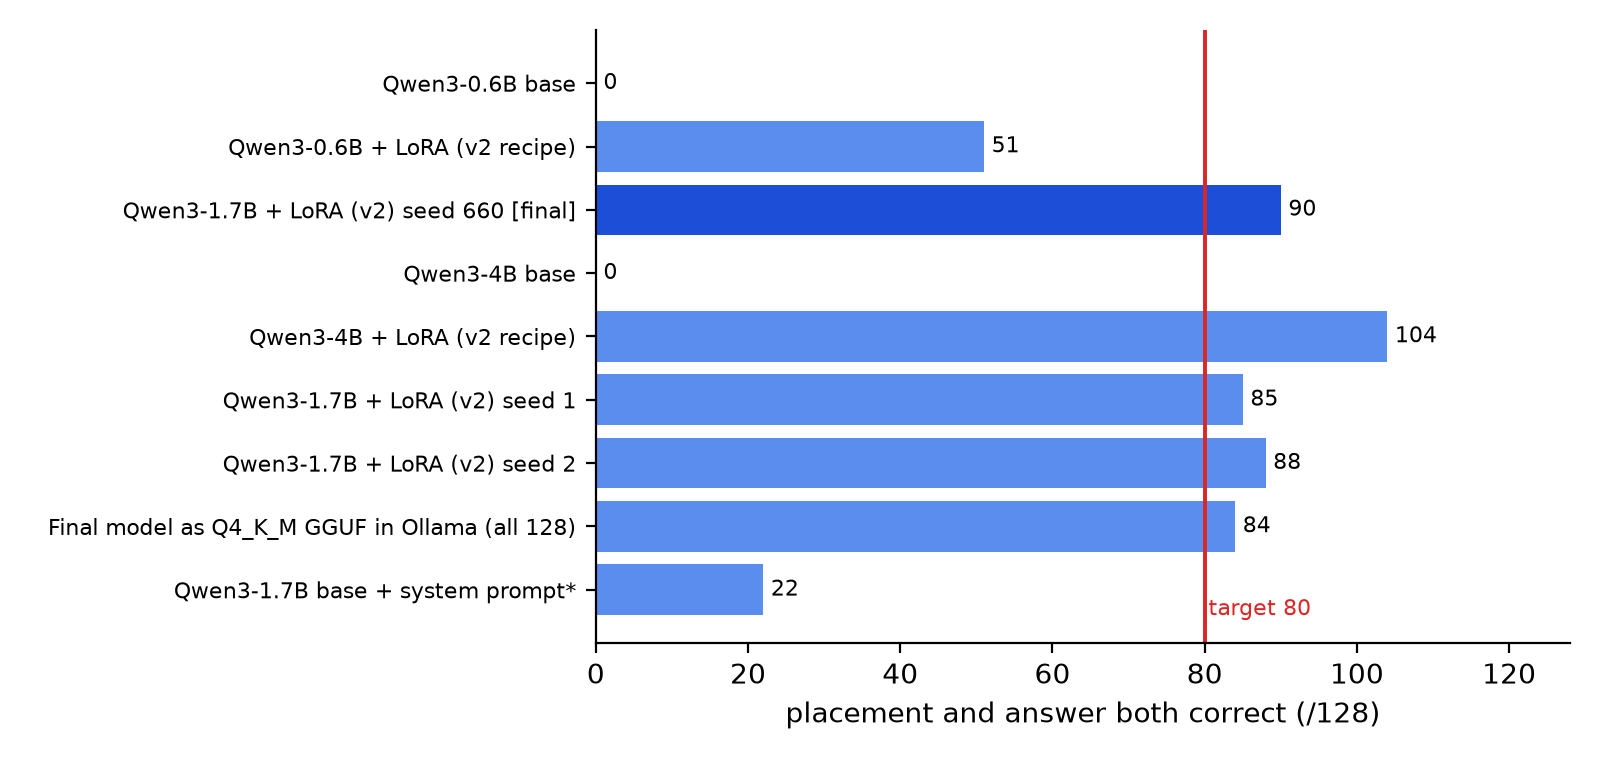
\includegraphics[width=0.8\linewidth]{figures/extra_experiments.png}
\caption{Placement and answer both correct for each extra run.}
\end{figure}
\paragraph{Findings.}
\begin{itemize}
\item \textbf{Fine-tuning is necessary.} Writing the rule in a system prompt gives only 22/128 both correct.
The base model writes the phrase inline (39 replies), repeats it, or puts it last on keep requests (27 false opt-outs). The LoRA adapter gets 90/128 without any instructions at inference.
\item \textbf{The result is robust to the seed.} Seeds 660, 1 and 2 all meet all five targets: both correct 90, 85 and 88 (mean 87.7). Opt-out recall varies most (41--43), and seeds 1 and 2 trade a few more false opt-outs (6, 8) for more caught opt-outs.
\item \textbf{Model size.} The same recipe on Qwen3-4B reaches 104/128 both correct, with 115/128 correct answers and only 1 false opt-out, at twice the memory (8.6\,GB, still within 16\,GB) and three times the training time.
Qwen3-0.6B learns the placement (73/80 first) but its answer accuracy \emph{drops} below its own base model (74 to 66): it has too little capacity to learn the format without forgetting content.
Qwen3-1.7B is the smallest size that meets every target.
\item \textbf{Quantisation cost.} On all 128 prompts the Q4\_K\_M GGUF loses 6 both-correct items (90 to 84) and 4 answers (97 to 93), but still meets every target.
\end{itemize}

\paragraph{Testing.} \texttt{tests/test\_score.py} contains 14 unit tests for the scorer: placement edge cases (whitespace, missing, repeated, inline, phrase inside JSON, wrong case), the prefix/suffix mapping, accepted equivalents, whole-token number matching, JSON key and type checks, and agreement between the summaries and a recount of the per-prompt rows.
Writing these tests caught one scorer bug: \texttt{9} matched inside \texttt{9.5}. I fixed it before reporting, and no reported number changed.

\section{Links (accessible to course staff)}
\begin{itemize}
\item Code, notebook, data (v1, v2 train/dev/dev\_heldout), run metadata, 3$\times$128 raw replies with per-prompt scores, dev replies, Ollama demo output: \LinkRepo
\item Final LoRA adapter (and initial adapter): \LinkAdapter
\item Q4\_K\_M GGUF, Modelfile and eight-prompt Ollama run: \LinkGGUF
\item Runnable notebook: \texttt{notebooks/DSEG660\_LoRA\_pipeline.ipynb} in the repository folder.
\end{itemize}
To reproduce, run \texttt{scripts/00\_setup\_env.sh}, then \texttt{01\_make\_data.py} (\texttt{--version v1}, then \texttt{v2}), \texttt{02\_train.py}, \texttt{07\_run\_eval.sh}, \texttt{05\_export\_gguf.sh} and \texttt{06\_ollama\_demo.py}.
The extra experiments are \texttt{08\_extra\_experiments.sh} and \texttt{09\_summarise.py}; the tests run with \texttt{pytest tests}. The exact commands are in the repository README.

\end{document}
